\documentclass[tikz,border=8pt]{standalone}

\usepackage{fontspec}
\setmonofont{Hack}

\usetikzlibrary{arrows.meta,backgrounds,calc,fit,positioning}

\begin{document}
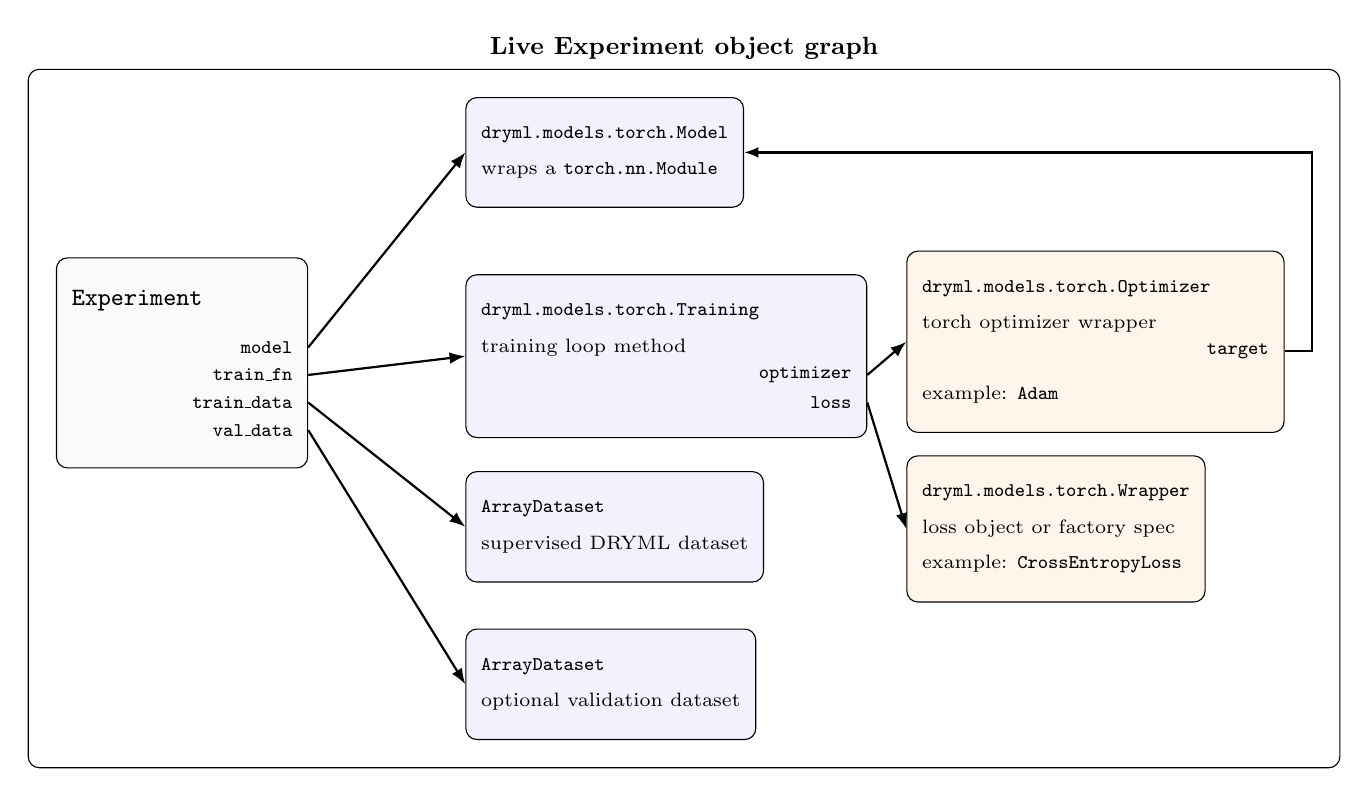
\begin{tikzpicture}[
  title/.style={font=\small\bfseries, anchor=west, align=left},
  object title/.style={font=\scriptsize\bfseries, anchor=west, align=left},
  attr/.style={font=\scriptsize, anchor=east, align=right},
  note/.style={font=\scriptsize, anchor=west, align=left},
  experiment box/.style={draw, rounded corners, inner xsep=2pt, inner ysep=8pt, fill=gray!4},
  object box/.style={draw, rounded corners, inner xsep=2pt, inner ysep=7pt, fill=blue!5},
  contained box/.style={draw, rounded corners, inner xsep=2pt, inner ysep=7pt, fill=orange!8},
  outer box/.style={draw, rounded corners, inner sep=10pt},
  relation/.style={-{Latex[length=2mm]},thick},
  dependency/.style={-{Latex[length=1.8mm]},thick}
]

% Column anchors. Each object gets a left text column and a right-justified
% attribute column. The fixed coordinates keep the rows from drifting.
\def\expLeft{0.0}
\def\expAttr{3.05}
\def\objLeft{5.2}
\def\objAttr{10.15}
\def\nestedLeft{10.8}
\def\nestedAttr{15.45}

% -----------------------------------------------------------------------------
% Column 1: Experiment object.
% -----------------------------------------------------------------------------
\node[title] (expTitle) at (\expLeft,0.9) {\texttt{Experiment}};
\node[attr] (expModel) at (\expAttr,0.3) {\texttt{model}};
\node[attr] (expTrainFn) at (\expAttr,-0.05) {\texttt{train\_fn}};
\node[attr] (expTrainData) at (\expAttr,-0.40) {\texttt{train\_data}};
\node[attr] (expValData) at (\expAttr,-0.75) {\texttt{val\_data}};

\begin{scope}[on background layer]
  \node[experiment box, fit=(expTitle)(expModel)(expTrainFn)(expTrainData)(expValData)] (expBox) {};
\end{scope}

% -----------------------------------------------------------------------------
% Column 2: objects referenced directly by Experiment attributes.
% -----------------------------------------------------------------------------
\node[object title] (modelTitle) at (\objLeft,3.0) {\texttt{dryml.models.torch.Model}};
\node[note] (modelType) at (\objLeft,2.55) {wraps a \texttt{torch.nn.Module}};
\begin{scope}[on background layer]
  \node[object box, fit=(modelTitle)(modelType)] (modelBox) {};
\end{scope}

\node[object title] (trainFnTitle) at (\objLeft,0.75) {\texttt{dryml.models.torch.Training}};
\node[note] (trainFnType) at (\objLeft,0.30) {training loop method};
\node[attr] (trainFnOptimizer) at (\objAttr,-0.05) {\texttt{optimizer}};
\node[attr] (trainFnLoss) at (\objAttr,-0.40) {\texttt{loss}};
\begin{scope}[on background layer]
  \node[object box, fit=(trainFnTitle)(trainFnType)(trainFnOptimizer)(trainFnLoss)] (trainFnBox) {};
\end{scope}

\node[object title] (trainDataTitle) at (\objLeft,-1.75) {\texttt{ArrayDataset}};
\node[note] (trainDataType) at (\objLeft,-2.20) {supervised DRYML dataset};
\begin{scope}[on background layer]
  \node[object box, fit=(trainDataTitle)(trainDataType)] (trainDataBox) {};
\end{scope}

\node[object title] (valDataTitle) at (\objLeft,-3.75) {\texttt{ArrayDataset}};
\node[note] (valDataType) at (\objLeft,-4.20) {optional validation dataset};
\begin{scope}[on background layer]
  \node[object box, fit=(valDataTitle)(valDataType)] (valDataBox) {};
\end{scope}

% -----------------------------------------------------------------------------
% Column 3: objects nested under train_fn.
% -----------------------------------------------------------------------------
\node[object title] (optimizerTitle) at (\nestedLeft,1.05) {\texttt{dryml.models.torch.Optimizer}};
\node[note] (optimizerType) at (\nestedLeft,0.60) {torch optimizer wrapper};
\node[attr] (optimizerTarget) at (\nestedAttr,0.25) {\texttt{target}};
\node[note] (optimizerExample) at (\nestedLeft,-0.30) {example: \texttt{Adam}};
\begin{scope}[on background layer]
  \node[contained box, fit=(optimizerTitle)(optimizerType)(optimizerTarget)(optimizerExample)] (optimizerBox) {};
\end{scope}

\node[object title] (lossTitle) at (\nestedLeft,-1.55) {\texttt{dryml.models.torch.Wrapper}};
\node[note] (lossType) at (\nestedLeft,-2.00) {loss object or factory spec};
\node[note] (lossExample) at (\nestedLeft,-2.45) {example: \texttt{CrossEntropyLoss}};
\begin{scope}[on background layer]
  \node[contained box, fit=(lossTitle)(lossType)(lossExample)] (lossBox) {};
\end{scope}

% -----------------------------------------------------------------------------
% Attribute-aligned connection points: arrows leave the box boundary beside the
% corresponding attribute row.
% -----------------------------------------------------------------------------
\coordinate (expModelOut) at (expBox.east |- expModel.east);
\coordinate (expTrainFnOut) at (expBox.east |- expTrainFn.east);
\coordinate (expTrainDataOut) at (expBox.east |- expTrainData.east);
\coordinate (expValDataOut) at (expBox.east |- expValData.east);

\coordinate (trainFnOptimizerOut) at (trainFnBox.east |- trainFnOptimizer.east);
\coordinate (trainFnLossOut) at (trainFnBox.east |- trainFnLoss.east);
\coordinate (optimizerTargetOut) at (optimizerBox.east |- optimizerTarget.east);
\coordinate (optimizerTargetBend) at ($(optimizerTargetOut)+(0.35,0)$);

\draw[relation] (expModelOut) -- (modelBox.west);
\draw[relation] (expTrainFnOut) -- (trainFnBox.west);
\draw[relation] (expTrainDataOut) -- (trainDataBox.west);
\draw[relation] (expValDataOut) -- (valDataBox.west);

\draw[relation] (trainFnOptimizerOut) -- (optimizerBox.west);
\draw[relation] (trainFnLossOut) -- (lossBox.west);
\draw[dependency] (optimizerTargetOut) -- (optimizerTargetBend) |- (modelBox.east);

\begin{scope}[on background layer]
  \node[outer box, fit=(expBox)(modelBox)(trainFnBox)(trainDataBox)(valDataBox)(optimizerBox)(lossBox)(optimizerTargetBend), label={[font=\bfseries\small]above:Live Experiment object graph}] {};
\end{scope}

\end{tikzpicture}
\end{document}
